\section{Design and Implementation}
\label{sec:desaindanimplementasi}

\subsection{System Description}
\label{sec:deskripsisistem}

\begin{figure}[ht]
  \centering
  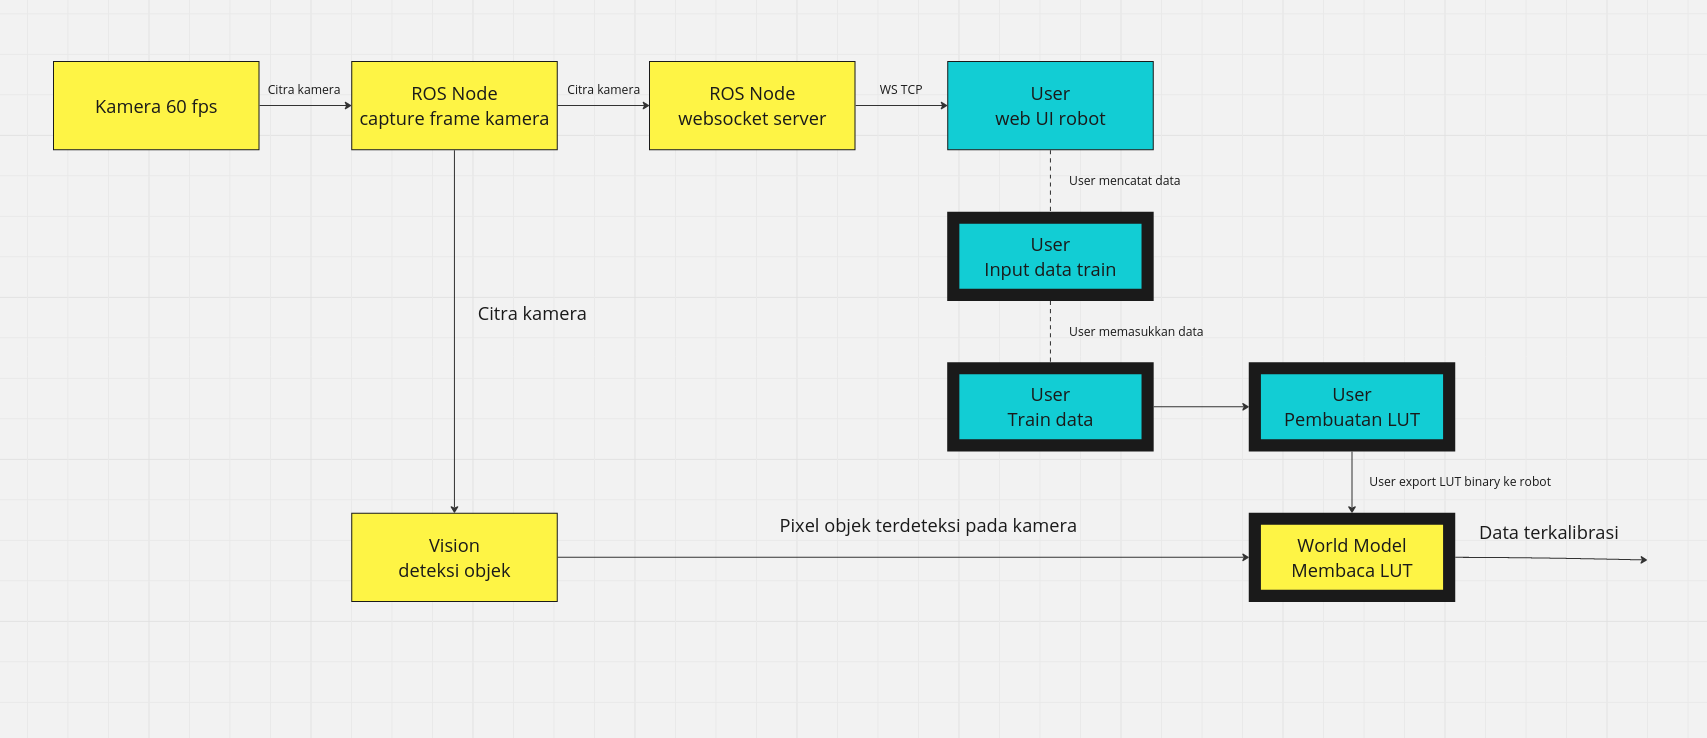
\includegraphics[width=8cm]{gambar/desain_sistem_vfix.png}
  \caption{Design System Block.}
  \label{fig:webrobot}
\end{figure}

From the figure above, the system is divided into two colors, namely yellow and cyan. The yellow color indicates that the process is running on the robot, while the cyan color indicates that the process is running outside the robot. The calibration system focuses on the system marked with a thick border, namely Data Retrieval, Data Training, Creating a Lookup Table, and the last is reading data from the Lookup Table so that it becomes calibrated data.

\subsection{Data Retrieval
  \label{sec:pengambilandata}}

The first thing to do before retrieving data is to prepare the robot and the marker that has been made before. The data taken is polar coordinate data both on the camera and on the field. The following formula is used to calculate polar coordinates on the camera:

\begin{equation}
  \begin{aligned}
    dx &= x - x\_center\_cam \\ 
    dy &= y\_center\_cam - y \\
    r &= \sqrt{dx^2 + dy^2} \\
    \theta &= \arctan(\frac{dy}{dx})
  \end{aligned}
\end{equation}

\begin{figure}[ht]
  \centering
  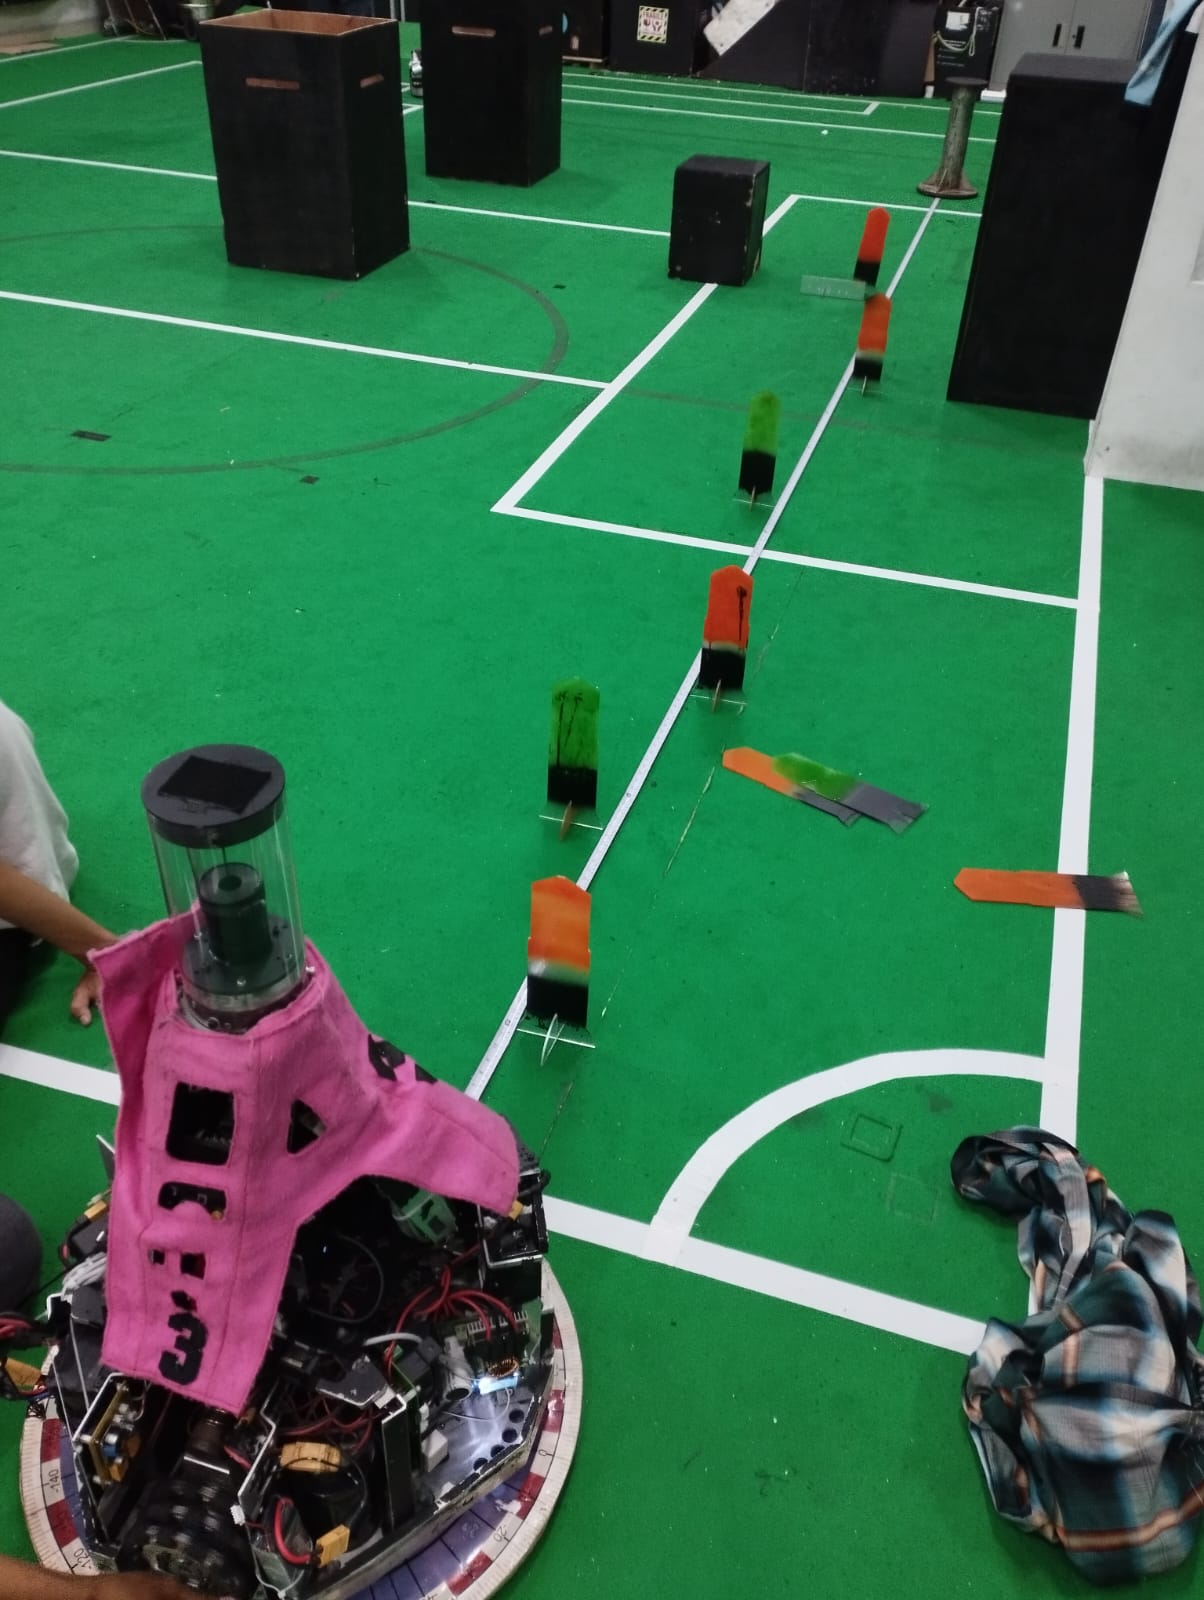
\includegraphics[width=5cm]{gambar/ambil_data.jpeg}
  \caption{Robot preparation.}
  \label{fig:persiapanrobot}
\end{figure}

Because the robot does not have a display, to access the camera needs to be done by accessing through the web program provided by the robot. The following is the view of robot camera displayed on the website.

\begin{figure}[ht]
  \centering
  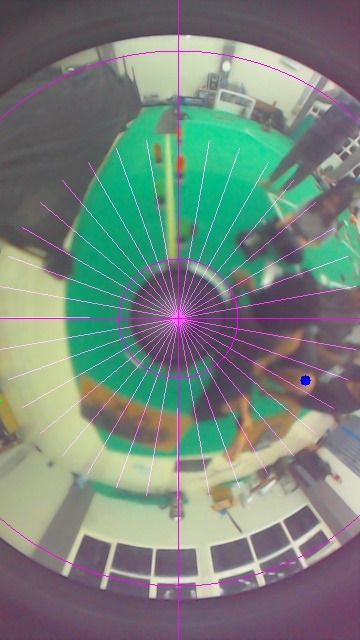
\includegraphics[width=5cm]{gambar/iris_web.jpeg}
  \caption{Robot camera display.}
  \label{fig:webrobot}
\end{figure}

From the website display, the red color on the field can be clicked and the polar coordinates on the camera will appear (according to the formula \textbf{3.1}). Then the coordinates will be saved to a file. The data taken is as follows:

\begin{table}[htbp]
  \caption{Training data.}
  \begin{center}
  \begin{tabular}{|c|c|c|}
    \hline
    \rowcolor[HTML]{C0C0C0}
    \textbf{Theta frame} & \textbf{Distance frame} & \textbf{Field distance} \\
    \hline
    0 deg            & 123.612 px                & 110 cm            \\
    0 deg           & 148.355 px                & 160 cm            \\
    0 deg           & 162.01 px                & 210 cm            \\
    0 deg           & 171.009 px                & 260 cm           \\
    10 deg           & 149.684 px                & 160 cm           \\
    19 deg           & 162.706 px                & 210 cm           \\
    10 deg           & 171.878 px                & 260 cm           \\
    20 deg           & 127.343 px                & 110 cm           \\
    20 deg           & 149.378 px                & 160 cm           \\
    20 deg           & 162.029 px                & 210 cm           \\
    20 deg           & 173.398 px                & 260 cm           \\
    ...           & ...                & ...           \\
    350 deg           & 147.681 px                & 160 cm           \\
    350 deg           & 159.797 px                & 210 cm           \\
    350 deg           & 169.577 px                & 260 cm           \\
    \hline
  \end{tabular}
  \label{tab1}
  \end{center}
\end{table}


\subsection{Training data
  \label{sec:trainingdata}}

The data that has been taken is then processed using the data training program. This program uses the Neural Network method to process the data. The following is the data training program.

The full architecture of the Neural Network used is having 2 hidden layers with 36 and 36 neurons each. The activation function used is Sigmoid with the formula as follows:

\begin{equation}
  \begin{aligned}
    f(x) &= \frac{1}{1 + e^{-x}}
  \end{aligned}
\end{equation}

The advantage of using Sigmoid is because Sigmoid has a value range between 0 and 1 which is suitable for the data to be processed.

The loss function used is the Mean Squared Error with the formula as follows:

\begin{equation}
  \begin{aligned}
    L(y, \hat{y}) &= \frac{1}{n} \sum_{i=1}^{n} (y_i - \hat{y_i})^2
  \end{aligned}
\end{equation}

The optimizer used is Adam with a learning rate of 0.0001.

The epoch used is 300000 times. It can change depending on the state of the data being trained.

The full architecture of the Neural Network used is as follows:

\begin{itemize}
    \item \( \mathbf{x} \in \mathbb{R}^2 \): Input data
    \item \( \mathbf{W}^{(1)} \in \mathbb{R}^{36 \times 2} \): weight layer 1
    \item \( \mathbf{b}^{(1)} \in \mathbb{R}^{36} \): bias layer 1
    \item \( \mathbf{W}^{(2)} \in \mathbb{R}^{36 \times 36} \): weight layer 2
    \item \( \mathbf{b}^{(2)} \in \mathbb{R}^{36} \): bias layer 2
    \item \( \mathbf{W}^{(3)} \in \mathbb{R}^{1 \times 36} \): weight layer 3
    \item \( \mathbf{b}^{(3)} \in \mathbb{R}^{1} \): bias layer 3
    \item \( \sigma \): sigmoid activation function
\end{itemize}

\begin{equation}
  \textbf{Input to Hidden Layer 1}:
  \begin{aligned}
    \mathbf{z}^{(1)} &= \mathbf{W}^{(1)} \mathbf{x} + \mathbf{b}^{(1)} \\
    \mathbf{a}^{(1)} &= \sigma(\mathbf{z}^{(1)})
  \end{aligned}
\end{equation}

\begin{equation}
  \textbf{Hidden Layer 1 to Hidden Layer 2}:
  \begin{aligned}
    \mathbf{z}^{(2)} &= \mathbf{W}^{(2)} \mathbf{a}^{(1)} + \mathbf{b}^{(2)} \\
    \mathbf{a}^{(2)} &= \sigma(\mathbf{z}^{(2)})
  \end{aligned}
\end{equation}

\begin{equation}
  \textbf{Hidden Layer 2 to Output Layer}:
  \begin{aligned}
    \mathbf{z}^{(3)} &= \mathbf{W}^{(3)} \mathbf{a}^{(2)} + \mathbf{b}^{(3)} \\
    \mathbf{a}^{(3)} &= \mathbf{z}^{(3)}
  \end{aligned}
\end{equation}

\subsection{Creating a Lookup Table
  \label{sec:pembuatanlut}}

After the data is trained, the data will be made into a Lookup Table. This Lookup Table contains the data that has been trained before. The following is the formula for creating a 2-dimensional Lookup Table:

\begin{equation}
  \begin{aligned}
    size &= \theta\_max \times r\_max \\
    index &= \theta \times r\_max + r
  \end{aligned}
\end{equation}

From the formula above, the size of the Lookup Table to be created and the index of the data to be entered into the Lookup Table can be obtained.
Then for the value of the Lookup Table itself comes from the formula \textbf{3.4 - 3.6}. These values will be entered into the Lookup Table according to the index calculated earlier.

\subsection{Reading the Lookup Table
  \label{sec:pembacaanlut}}

After the Lookup Table is created, the last thing is to read data from the Lookup Table with the formula as follows.

\begin{equation}
  \begin{aligned}
    index &= \theta\_cam \times r\_max + r\_cam \\
    r\_real &= \text{Lookup\_Table}[index] \\
    \theta\_real &= \theta\_cam
  \end{aligned}
\end{equation}

This process is done on the robot. The following is the Lookup Table reading program.





